\documentclass[12pt,draft]{article}

% Allow block comment commands
\usepackage{comment}

\begin{comment}
draft - disables image rendering, shows black boxes at hyphenation issues

Defaults:
	10pt
	notitlepage
	a4paper (usletter on some distros)
	singleside (twoside changes the margins for a binding)

Style:
http://practicaltypography.com
https://www.sharelatex.com/learn/Paragraphs_and_new_lines

title styling
http://texblog.org/2012/07/03/fancy-latex-chapter-styles/

Left-aligned text; equal spacing between words, better readability
	May look "unprofessional", books, articles typically use fully justified
	ragged2e retains hyphenation and attempts to give a more uniform right edge, but maintains equal spacing between words
\end{comment}
\usepackage[document]{ragged2e}
% Adjust default length before hyphenation, reducing amount of hyphenation
\setlength{\RaggedRightRightskip}{0pt plus 3.5em}
\raggedright


% Single space after a full stop, modern typographic readability standard
\frenchspacing

% Paragraph spacing with no indent; breaks up huge blocks of text
\usepackage{parskip}

% Line spacing (Default or slightly larger?)
\usepackage{setspace}
%\onehalfspacing

% Header and footer
\usepackage{fancyhdr}
\fancyhead[L]{\nouppercase{\textbf{\rightmark}}}
\fancyhead[R]{\textbf{\thepage}}
\cfoot{}
\renewcommand{\headrulewidth}{0.5pt}
%\renewcommand{\footrulewidth}{0.5pt}

% Roman section numbering, numbered subsections
\renewcommand \thesection{\Roman{section}}
\renewcommand \thesubsection{\arabic{section}.\arabic{subsection}}

% Page decorations
% Adapted from: http://tex.stackexchange.com/questions/85904/showcase-of-beautiful-title-page-done-in-tex
\usepackage{tikz}

% Colour scheme
\definecolor{pagecolour}{cmyk}{1,.60,0,.40}

% Right side decorations
\newcommand\pagedecorationright{
\begin{tikzpicture}[remember picture,overlay,shorten >= -10pt]

\coordinate (aux1) at ([yshift=-15pt]current page.north east);
\coordinate (aux2) at ([yshift=-410pt]current page.north east);
\coordinate (aux3) at ([xshift=-4.5cm]current page.north east);
\coordinate (aux4) at ([yshift=-150pt]current page.north east);

\begin{scope}[pagecolour!40,line width=12pt,rounded corners=12pt]
\draw
  (aux1) -- coordinate (a)
  ++(225:5) --
  ++(-45:5.1) coordinate (b);
\draw[shorten <= -10pt]
  (aux3) --
  (a) --
  (aux1);
\draw[opacity=0.6,pagecolour,shorten <= -10pt]
  (b) --
  ++(225:2.2) --
  ++(-45:2.2);
\end{scope}
\draw[pagecolour,line width=8pt,rounded corners=8pt,shorten <= -10pt]
  (aux4) --
  ++(225:0.8) --
  ++(-45:0.8);
\begin{scope}[pagecolour!70,line width=6pt,rounded corners=8pt]
\draw[shorten <= -10pt]
  (aux2) --
  ++(225:3) coordinate[pos=0.45] (c) --
  ++(-45:3.1);
\draw
  (aux2) --
  (c) --
  ++(135:2.5) --
  ++(45:2.5) --
  ++(-45:2.5) coordinate[pos=0.3] (d);   
\draw 
  (d) -- +(45:1);
\end{scope}
\end{tikzpicture}
}

% Left side decorations
\newcommand\pagedecorationleft{
\begin{tikzpicture}[remember picture,overlay,shorten >= -10pt]
\coordinate (aux1) at ([yshift=-15pt]current page.north west);
\coordinate (aux2) at ([yshift=-410pt]current page.north west);
\coordinate (aux3) at ([xshift= 4.5cm]current page.north west);
\coordinate (aux4) at ([yshift=-150pt]current page.north west);

\begin{scope}[pagecolour!40,line width=12pt,rounded corners=12pt]
\draw
  (aux1) -- coordinate (a)
  ++(-45:5) --
  ++(-135:5.1) coordinate (b);
\draw[shorten <= -10pt]
  (aux3) --
  (a) --
  (aux1);
\draw[opacity=0.6,pagecolour,shorten <= -10pt]
  (b) --
  ++(-45:2.2) --
  ++(-135:2.2);
\end{scope}
\draw[pagecolour,line width=8pt,rounded corners=8pt,shorten <= -10pt]
  (aux4) --
  ++(-45:0.8) --
  ++(-135:0.8);
\begin{scope}[pagecolour!70,line width=6pt,rounded corners=8pt]
\draw[shorten <= -10pt]
  (aux2) --
  ++(-45:3) coordinate[pos=0.135] (c) --
  ++(-135:3.1);
\draw
  (aux2) --
  (c) --
  ++(45:2.5) --
  ++(135:2.5) --
  ++(-135:2.5) coordinate[pos=0.3] (d);   
\draw 
  (d) -- +(135:1);
\end{scope}
\end{tikzpicture}
}
\definecolor{pagecolour}{cmyk}{1,.60,0,.40}

% Font choices - LaTeX default is computer modern, a bit thin for my liking
% https://www.tug.org/mactex/fonts/LaTeX_Preamble-Font_Choices.html
% Palatino body text
%\renewcommand{\rmdefault}{ppl}
%\linespread{1.05}

% Tools
\usepackage{mathtools}
\usepackage{graphicx}
\usepackage{epstopdf}
\usepackage{siunitx}
\usepackage{acronym}
\usepackage{hyperref}
% In text subscripts and superscripts
\usepackage{fixltx2e}

% Some handy commands for referencing (copied from old template)
\newcommand{\figref}[2][\figurename~]{#1\ref{#2}}
\newcommand{\tabref}[2][\tablename~]{#1\ref{#2}}
\newcommand{\secref}[2][Section~]{#1\ref{#2}}
\renewcommand{\vec}[1]{\mathbf{#1}}

\begin{comment}
Useful LaTeX commands/tools:
	\clearpage ends the current page and causes all figures and tables that have so far appeared in the input to be printed.
	www.doi2bib.org

General writing tips:
https://owl.english.purdue.edu/owl/section/1/2/
	3-5 sentences per paragraph; one idea, contrast, a break, balance
	15-20 words per sentence; comprehension lowers the longer it gets
	25-33 syllables; most like typical speech
	50-75 characters per line, ~65 seems optimal
	Use plain English; simpler words are better words
	Explain all technical jargon and abbreviations at first use

Science writing:
	Figure text and the abstract should be independent from main text
	List assumptions after each sub-theory (being clear about problems)
	Every review is gold dust, people can only read the first time once
	Send your draft to your references to see if you've cited their work fairly

\end{comment}

\begin{document}

%Front Matter

% Remove page numbering
\pagenumbering{garble}
\pagestyle{empty}

% Fancy title page, modified version of fancy-title.tex
\begin{titlepage}
\center
% Headings
\textsc{\huge University of Exeter}\\[1cm]
\textsc{\Large MPhys Project}\\[1.5cm]
%\textsc{\large Minor Heading}\\[0.5cm]

% Title
\rule{\linewidth}{0.5mm}\\[0.4cm]
\begin{doublespace}
{\LARGE \textbf{Thermoelectric Efficiency of Zero-dimensional Nanocomposites}}\\[0cm]
\end{doublespace}
\rule{\linewidth}{0.5mm}\\[2.5cm]
 
% Authors
\begin{minipage}{0.4\textwidth}
\begin{flushleft} \large
\emph{Author:}\\
Callum \textsc{Vincent}
\end{flushleft}
\end{minipage}
~
\begin{minipage}{0.4\textwidth}
\begin{flushright} \large
\emph{Supervisor:} \\
Prof. G. P. \textsc{Srivastava}
\end{flushright}
\end{minipage}\\[4cm]

% Date
{\large April 2015}

\pagedecorationleft
\pagedecorationright
\end{titlepage}

% Abstract page
\begin{center}
{\Huge\textbf{Abstract}}\\[2cm]
\end{center}
\begin{justify}
Thermoelectrics are currently limited by their heat to electric conversion efficiency. If their efficiency can be improved 3$\times$ then a wide array of technological applications can be developed. Nanocomposite structuring is a potential technique for achieving this. We utilise an effective medium approximation to calculate the thermoelectric efficiency of a zero-dimensional SiGe nanocomposite. We find that silicon spheres of 10nm diameter densely packed in a germanium host medium, improves the thermoelectric efficiency 2.6$\times$ compared to bulk SiGe. This gives good indiciation that further theoretical and experimental research should be conducted.
\end{justify}

\pagebreak

\tableofcontents

\pagebreak

% Main text

% Set numeric page numbering
\pagestyle{fancy}
\pagenumbering{arabic}

\section{Introduction}
% Review previous research
 
\subsection{Motivation}
% Why would you want do this?
Energy and its use defines human society. Throughout history we have seen an upwards trend of energy consumption and with it we transform our environment and our lives.

Thermoelectric materials have the potential to revolutionise our energy harvesting methods due to their ability to convert heat directly into electricity. This potential has motivated decades of research, resulting in; radioisotope thermonuclear generators, solid state refrigerators and precise thermal control systems.

The main limitation of thermoelectric materials is their heat to electricity conversion efficiency. In modern applications, this is approximately 7\% \cite{modern-thermoelectrics}, roughly 4$\times$ lower than what is currently possible for internal combustion engines \cite{engine-efficiency}.

Recent advances in nano-fabrication have facilitated the development of new nanocomposite materials. Closely resembling metamaterials; nanocomposites are typically periodic arrays of nanoscale sheets, wires or particles. In 2001, it was shown that layering thin-films of thermoelectric materials gave a 2.4$\times$ increase in the thermoelectric figure of merit ZT \cite{nanocomposite-zt}; a key parameter in the conversion efficiency discussed above.

If ZT can be increased 3$\times$, an efficiency comparable to combustion engines could be attained in typical thermoelectric systems \cite{liu-review}. This would open up a wide array of applications such as: solar thermoelectric panels \cite{solar-thermal}, exhaust heat recovery systems \cite{exhust-recovery} and high reliability refrigeration systems \cite{thermo-cooling}.

It is therefore the goal of this project to understand how nanocomposite structuring effects the electrical and thermal properties of thermoelectric materials and whether a ZT\textgreater3 can be achieved.

\subsection{Approach}
% Describe the problem 
% Describe the idea
% Make claims about and defend the idea
Thermoelectricity requires a compromise between 3 variables; $S$ the Seebeck coefficient, $\sigma$ the electrical conductivity and $k$ the thermal conductivity. The thermoelectric figure of merit ZT and ultimately the conversion efficiency, is maximised when both $S$ and $\sigma$ are much greater than $k$. This is well shown in \figref{fig:zt-vs-doping}, where a decreasing $k$ and increasing $\sigma$ produce a maximum in ZT.

The problem therefore lies in the complex interplay between these 3 variables; how do we disentangle their relationships and produce a positive effect on ZT?

\begin{figure}
	\centering
	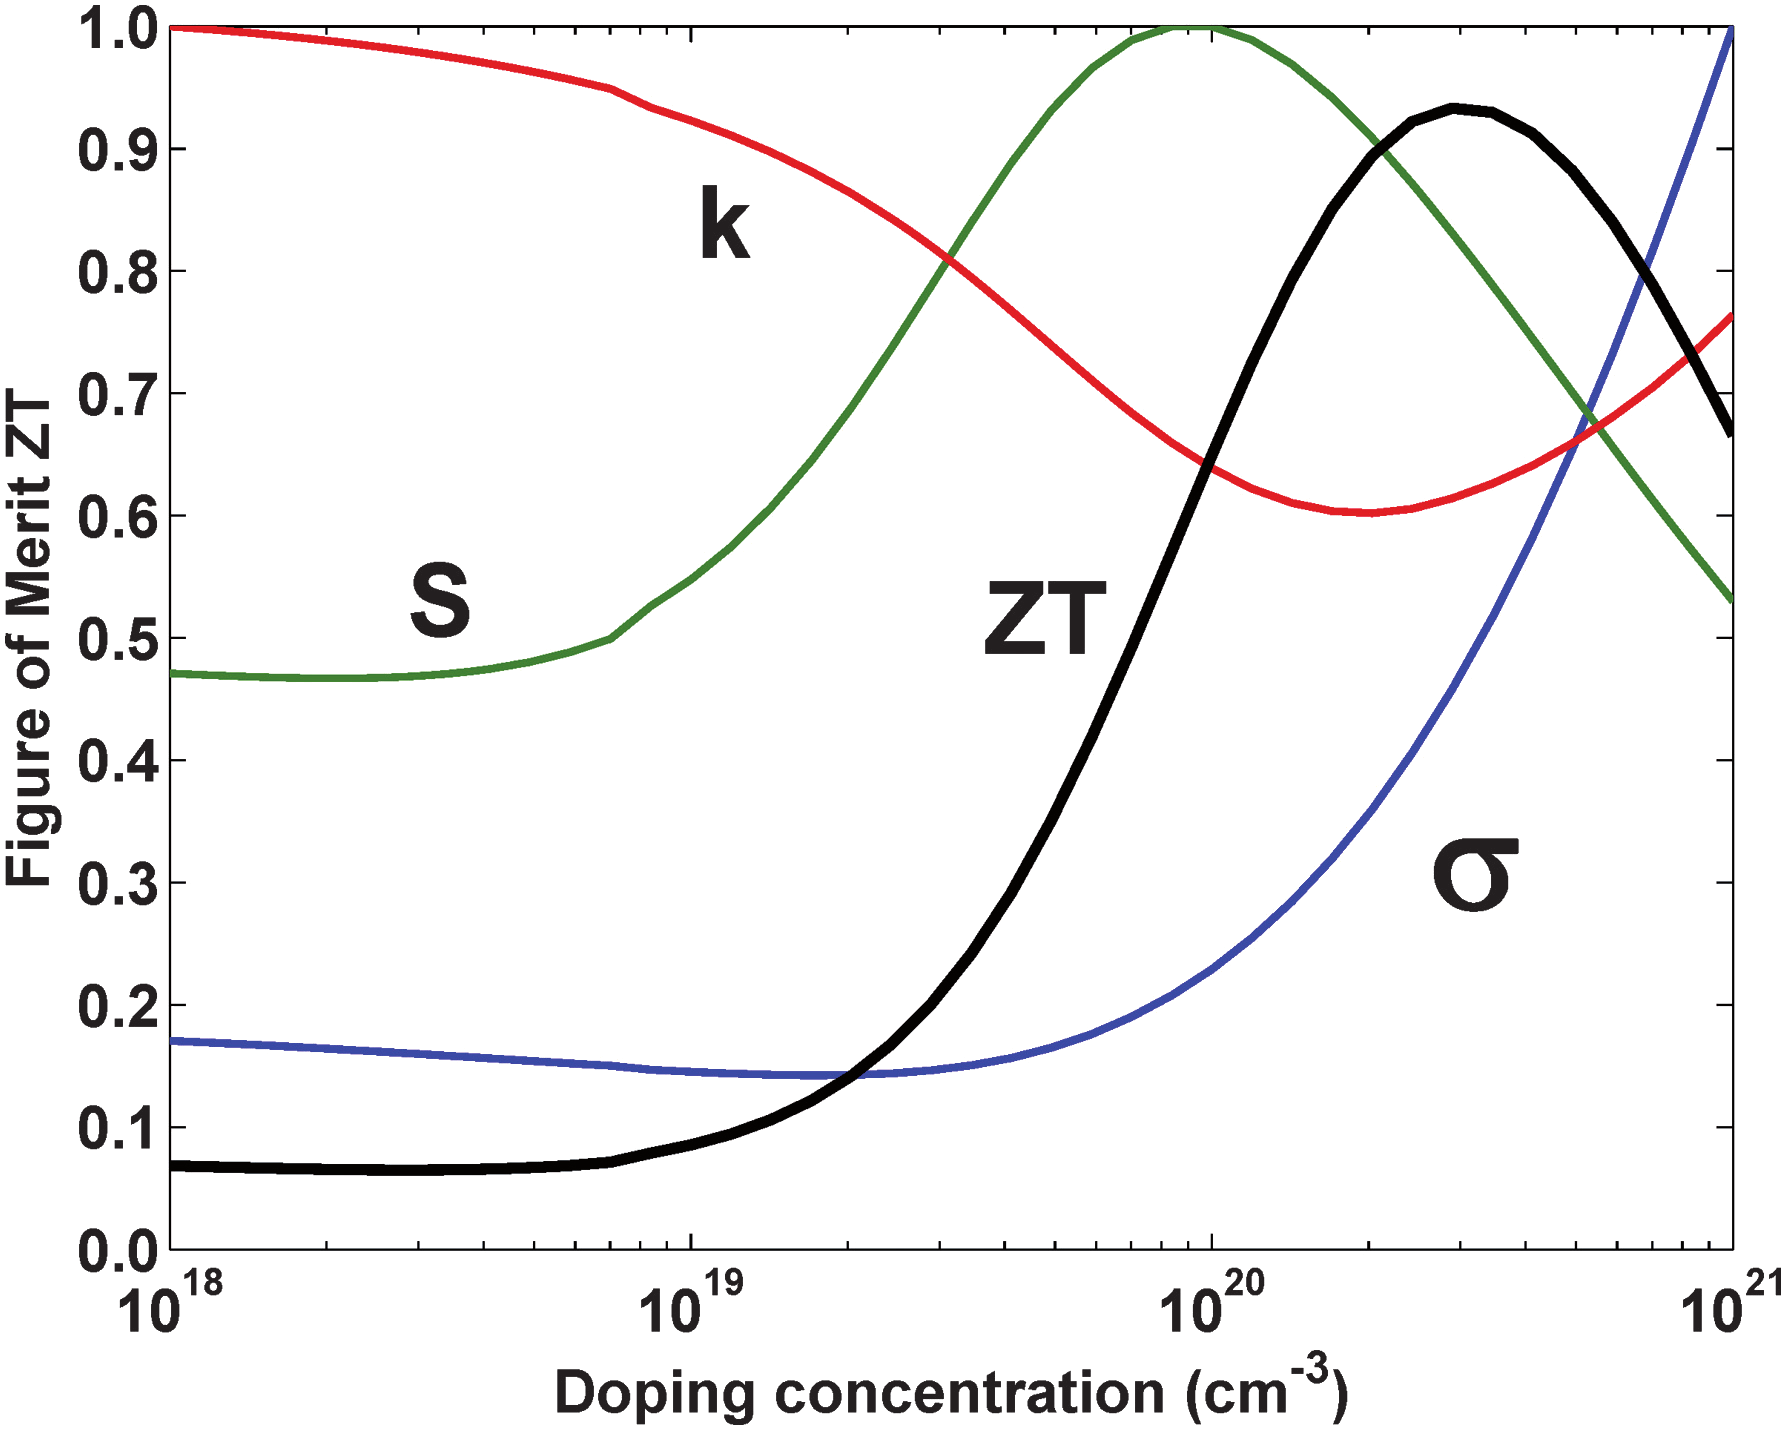
\includegraphics[width=0.8\textwidth]{zt-vs-doping.png}
	\caption{Normalised thermoelectric properties \emph{versus} doping concentration at 300 K for n-type Si\textsubscript{80}Ge\textsubscript{20} \cite{minnich-review}. Variables defined as follows: $S$ Seebeck coefficient, $\sigma$ electrical conductivity, $k$ thermal conductivity and ZT the thermoelectric figure of merit (proportional to conversion efficiency). The interrelationships between the variables gives a maximum ZT for a heavily doped semiconductor.}
	\label{fig:zt-vs-doping}
\end{figure}

In the \emph{CRC Handbook of Thermoelectrics} \cite{crc-handbook}, G. A. Slack proposes a mechanism for enhancing ZT, the phonon glass electron crystal (PGEC). In a PGEC, the material is structured to restrict phonon propagation (PG), but enhance electron propagation (EC). If these two effects are independent, then the resultant increase in electrical conductivity and decrease in thermal conductivity will boost ZT, as in \figref{fig:zt-vs-doping}.

In 1993, Hicks and Dresselhaus theoretically showed that a nanocomposite of closely packed nanoscale cylinders had the potential to significantly increase ZT \cite{nanowires}. We interpreted their findings to be in agreement with the PGEC concept; the cylinder boundaries are scattering phonons, whilst leaving the electrons unaffected. Therefore nanocomposite structuring may offer a possible technique for developing a PGEC material.

As a relatively new field, nanocomposites and its conceptual framework is still young and in development. In the context of thermoelectrics, theories for $S$, $\sigma$ and $k$ all need to be explored. We hypothesised that the main reason for the increase of ZT in nanocomposite structuring, is the scattering of phonons. So for our project, we decided to focus on $k$, specifically the phononic contribution $k_{ph}$. 

Of the literature reviewed, two theories for $k_{ph}$ were of note, the effective medium approximation (EMA) \cite{ema} and the phonon hopping model (PHM) \cite{phm}. The EMA considers a homogeneous host material whose phonon thermal conductivity is perturbed by a regularly arranged nanostructure. Whereas the PHM considers a linear chain of host atoms regularly perturbed by nanoparticles and calculates the probability of a phonon hopping past or interacting with these nanoparticles. We evaluated both models in detail and decided that the PHM neglected crucial thermoelectric properties, so we adopted the EMA for our calculations.

Our final consideration is which nanocomposite structure to investigate. Originally, we had planned to test multiple structures and compare their effects. However, as we were studying the EMA theory, it became clear that the optimum structure would have a high density of interfaces, with maximal gaps between these interfaces. This made closely packed spheres an ideal choice, as there is minimal contact between the spheres and a large surface area exposed to the host material. This structure is illustrated in \figref{fig:nanospheres-cube}.

\begin{figure}
	\centering
	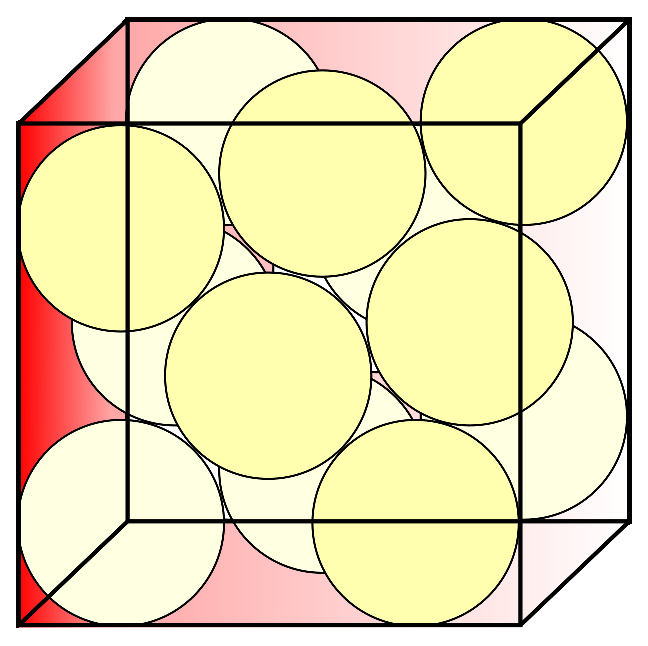
\includegraphics[width=0.5\textwidth]{nanospheres-cube.eps}
	\caption{Zero-dimensional nanocomposite structure. Nanoscale spheres are densely packed with a homogeneous host material filling the voids. A temperature gradient is shown, to illustrate use as a thermoelectric.}
	\label{fig:nanospheres-cube}
\end{figure}

\subsection{Investigation}
% Survey the paper, forward reference the interesting parts, make explicit your contributions to the problem
With the components discussed in the previous section


\section{Background Theory}
% Explain the intuition as if on a whiteboard
All the theories discussed in this report are transport processes. Therefore fundamental to them all are the non-equilibrium statistical mechanics of their quasiparticles.

\subsection{Boltzmann Equation}
The Boltzmann equation describes the statistical behaviour of a thermodynamic system of particles not in thermodynamic equilibrium and its general definition is:

\begin{equation}
\label{boltz-trans}
	\frac{\partial f}{\partial t} = \left(\frac{\partial f}{\partial
	t}\right)_\mathrm{force} + \left(\frac{\partial f}{\partial t}\right)_\mathrm{diff}+ \left(\frac{\partial f}{\partial t}\right)_\mathrm{coll}
\end{equation}

where $\frac{\partial f}{\partial t}$ is the time dependence of the distribution function of the particles $f$, the ``force" term represents external forces on the particles, the ``diff" term is the diffusion of particles through the system and the ``coll" term represents forces acting between particles in collisions.

From this general definition we can find how a particular system of particles or quasiparticles are distributed across a material and therefore find their average motion. We use this in the electrical conductivity $\sigma$ (\secref{electrical-conductivity}) and phonon thermal conductivity $k_{ph}$ (\secref{phonon-thermal}) derivations.

So we have a way of finding the distribution of our quasiparticles, but what exactly are the quasiparticles we are dealing with? And how are they important in the context of thermoelectrics?

\subsection{Phonons}

A phonon is the quantisation of vibrational motion of a lattice of atoms at a single frequency, known as a normal mode \cite{kittel}. These phonons are quasiparticles, free to move around the crystal lattice and they are distributed according to the Bose-Einstein distribution \cite{kittel}:

\begin{equation}
\label{bose-einstein}
	 \bar{n} = \frac{1}{e^{(\hbar \omega) / k T} - 1}
\end{equation}

where $\bar{n}$ is the probability of a phonon existing with energy $\hbar \omega$ at temperature $T$. This distribution is shown in \figref{3d-bose-einstein}

\begin{figure}
	\centering
	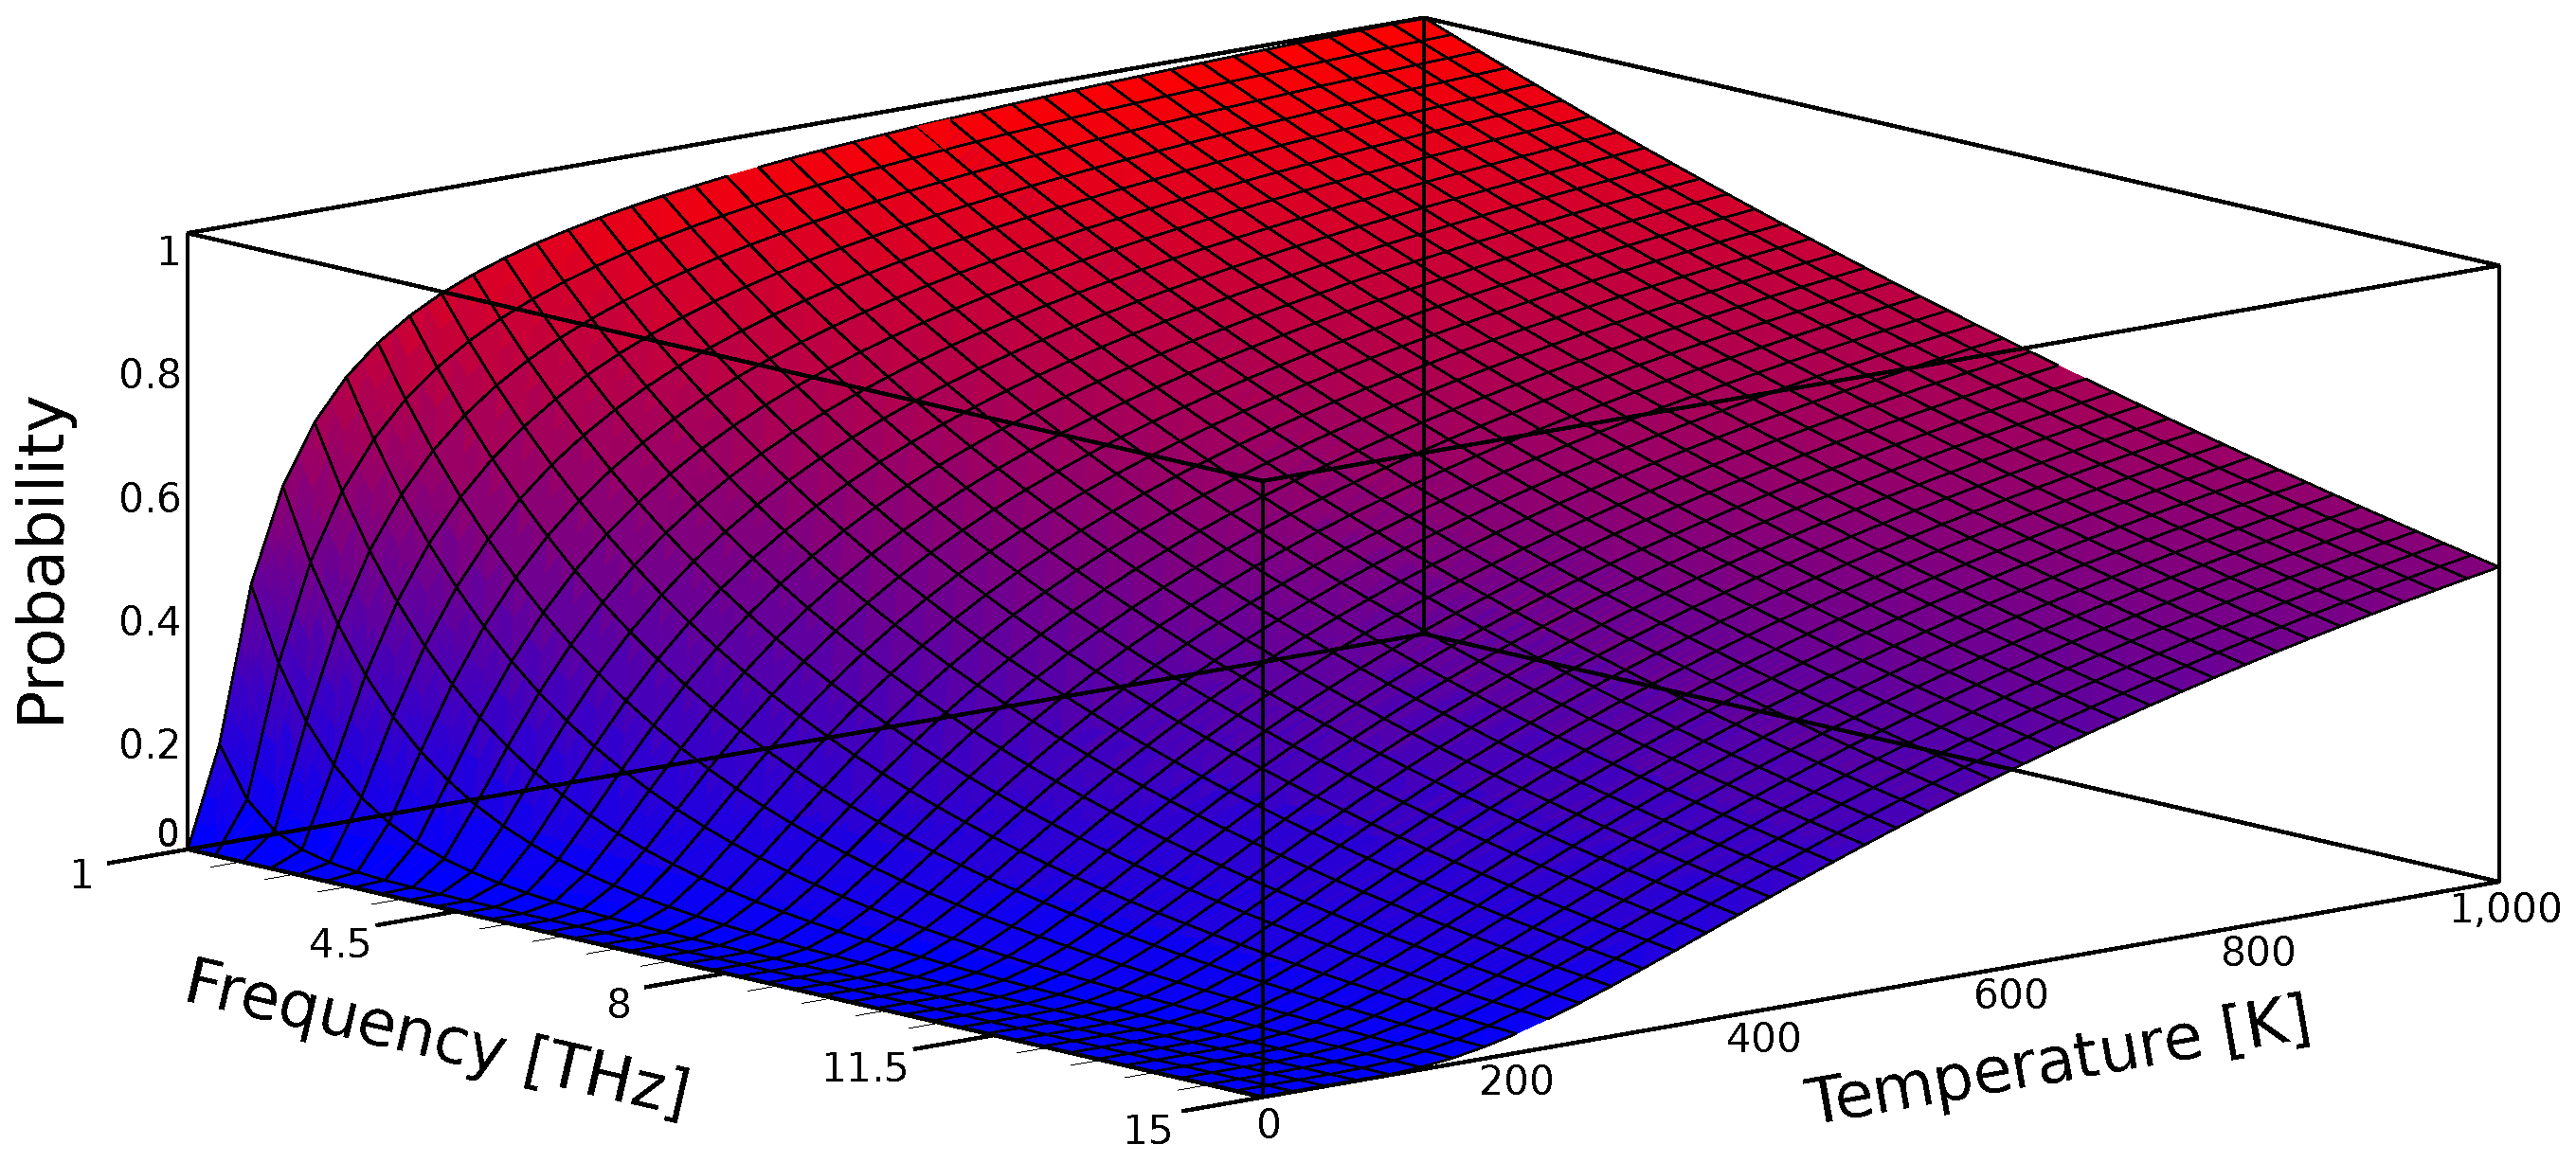
\includegraphics[width=\textwidth]{3d-bose-einstein.eps}
	\caption{Probability of phonon occupancy \emph{versus} phonon frequency and temperature.}
	\label{fig:3d-bose-einstein}
\end{figure}

Phonons are carriers of acoustic and thermal energy through a material. They follow two types of dispersion curve; optical and acoustic. For the energies of typical phonons around room temperature, we can neglect the optical branch, 

\paragraph{Assumptions}
\begin{itemize}
  \item Acoustic phonons
  \item 
  \item 
\end{itemize}



Electrons can be modelled as quasiparticles in a similar way, with a wavevector and effective mass as in equation \eqref{micro-elec}, leading to the Fermi-Dirac distribution \cite{kittel}:

\begin{equation}
\label{fermi-dirac}
	 \bar{f} = \frac{1}{e^{(E - E_f) / k T} + 1}
\end{equation}

where $\bar{f}$ is the probability of an electron existing with energy $E$ and $E_f$ is the Fermi level.

In the presence of an external fields, phonon and electron
distributions (\eqref{bose-einstein} \& \eqref{fermi-dirac}) both
satisfy the Boltzmann transport equation \eqref{boltz-trans} with \cite{ziman}:

\begin{equation}
\label{boltz-specific}
	\frac{df}{dt}\bigg|_{field} + \frac{df}{dt}\bigg|_{collisions} = 0
\end{equation}

where function $f$ is $f = \bar{n}$ or $f = \bar{f}$, the Bose-Einstein and Fermi-Dirac distribution functions.

\subsection{Thermoelectricity}
In 1821, Thomas Seebeck discovered that circuit made from two dissimilar metals, with junctions at different temperatures would deflect a compass magnet (\ref{seebeck-experiment}), he had discovered thermoelectricity. The temperature gradient $\vec{\nabla} T$ between the junctions generates an electromotive force:

\begin{equation}
\label{seebeck-emf}
	\vec{E_{emf}} = -S \vec{\nabla} T
\end{equation}

where $S$ is the Seebeck coefficient, defined as the induced voltage per unit temperature difference, mathematically $\Delta S = \frac{\Delta V}{\Delta T}$ \cite{auparay}. This coefficient is not only material dependent, but also temperature dependent, i.e., a temperature gradient produces an electromotive force gradient. This electromotive force gradient produces a current density gradient described macroscopically by a modified Ohm's law \cite{ziman}:

\begin{equation}
\label{current-density}
	\vec{J} = \sigma (-\vec{\nabla} V - S \vec{\nabla} T)
\end{equation}

where $\vec{J}$ and $\sigma$ are the current density $\frac{I}{A}$ and electrical conductivity at a given location in the material and $\vec{\nabla} T$ and $\vec{\nabla} V$ are the temperature and resultant voltage gradients across the material. If we were to repeat the experiment conducted by Seebeck (\figref{seebeck-experiment}), using a probe to measure $V$ between junctions and $\sigma$ at each junction for one of the metals, assuming steady state, i.e., $I=0$ so $\vec{J} = 0$, the metal's Seebeck coefficient can be determined.

Thermoelectricity, its uses and current nanocomposite research are well summarised by J. W. Bos \cite{bos-review} and A. J. Minnich \emph{et al.} \cite{minnich-review}.

\begin{figure}
	\centering
	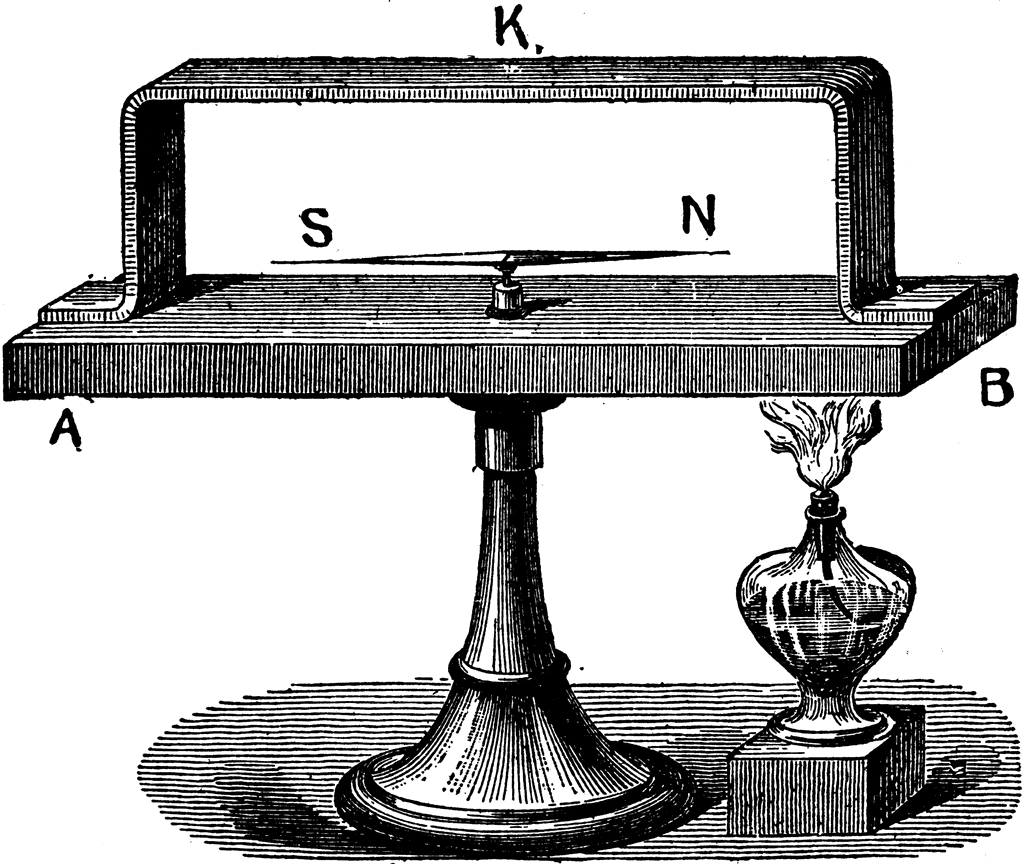
\includegraphics[width=\textwidth]{seebeck-experiment-black.png}
	\caption{Thomas Seebeck's original thermoelectricity experiment diagram \cite{seebeck-original}. A compass needle lies on top of one metal, underneath a bridge of a different metal (K), connected by two junctions and heated at one of these junctions.}
	\label{fig:seebeck-experiment}
\end{figure}

\subsection{Nanocomposites}
Composite materials are combinations of two or more materials, forming a new structure with significantly different physical or chemical properties than its constituent parts. In a similar way, nanocomposites are the structuring of multiple materials, but at the nanoscale. As our nanocomposites are at a comparable size to the crystal lattices of their constituent materials, we can view nanocomposites as artificial defects in a larger crystal lattice. A simple example of a 2D nanocomposite, a copper-graphene superlattice, is pictured in \figref{superlattice}. Examining one layer of th0e superlattice, the material in bulk form would be a 3D crystal structure, but by constraining the layer thickness we have introduced a boundary defect. The periodic array of these boundary defects forms a new 3D artificial crystal, which we define as a superlattice, a nanocomposite.

\begin{figure}
	\centering
	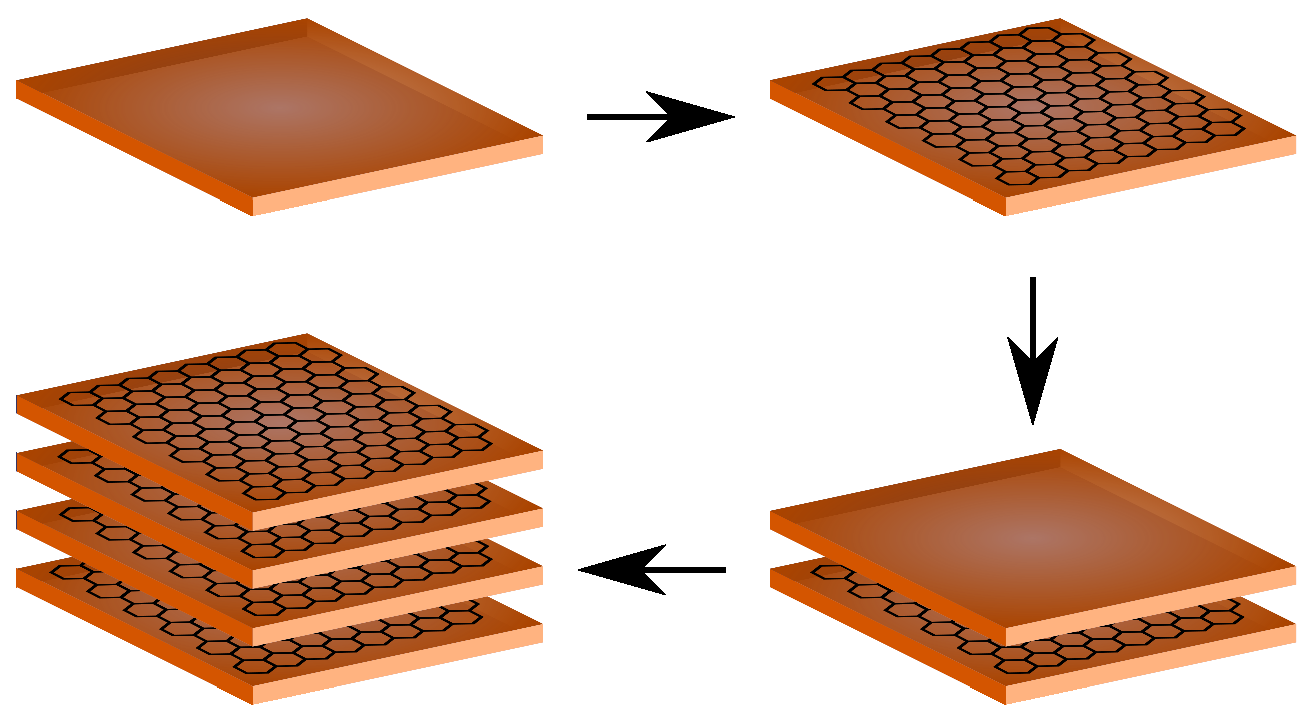
\includegraphics[width=\textwidth]{graphene-superlattice.eps}
	\caption{Superlattice of graphene and copper. Alternate layers of nanoscale copper and graphene are sandwiched together.}
	\label{fig:superlattice}
\end{figure}

\paragraph{Assumptions}

\section{Specific Theory}
% Details of exactly what you've done
% Tell a story, keep it concise, only explain what you need to
From a qualitative understanding, there must be strong boundary and interface effects; by definition nanocomposites contain numerous transitions between two or more materials, where each transition forms a new interface. Therefore a thorough understanding of how interfaces affect the propagation of phonons and electrons is required.

The EMA considers a homogeneous host material with a phonon thermal conductivity $k_h$, that is regularly perturbed by an interface resistance $R$ and separate phonon thermal conductivity $k_p$, which is then averaged over a relevant length scale $d$.

Some key questions for our project are; How can we achieve \ac{PGEC}? What are its constraints? How effective is it at increasing $ZT$?


\subsection{Thermoelectric Theory}
\paragraph{Assumptions}

\section{Results and Analysis}
% Split into two sections if lengthy
% Explain all elements leading to the results
% Include key graphs, have minimal tables
% What do they show?

\begin{figure}
	\centering
	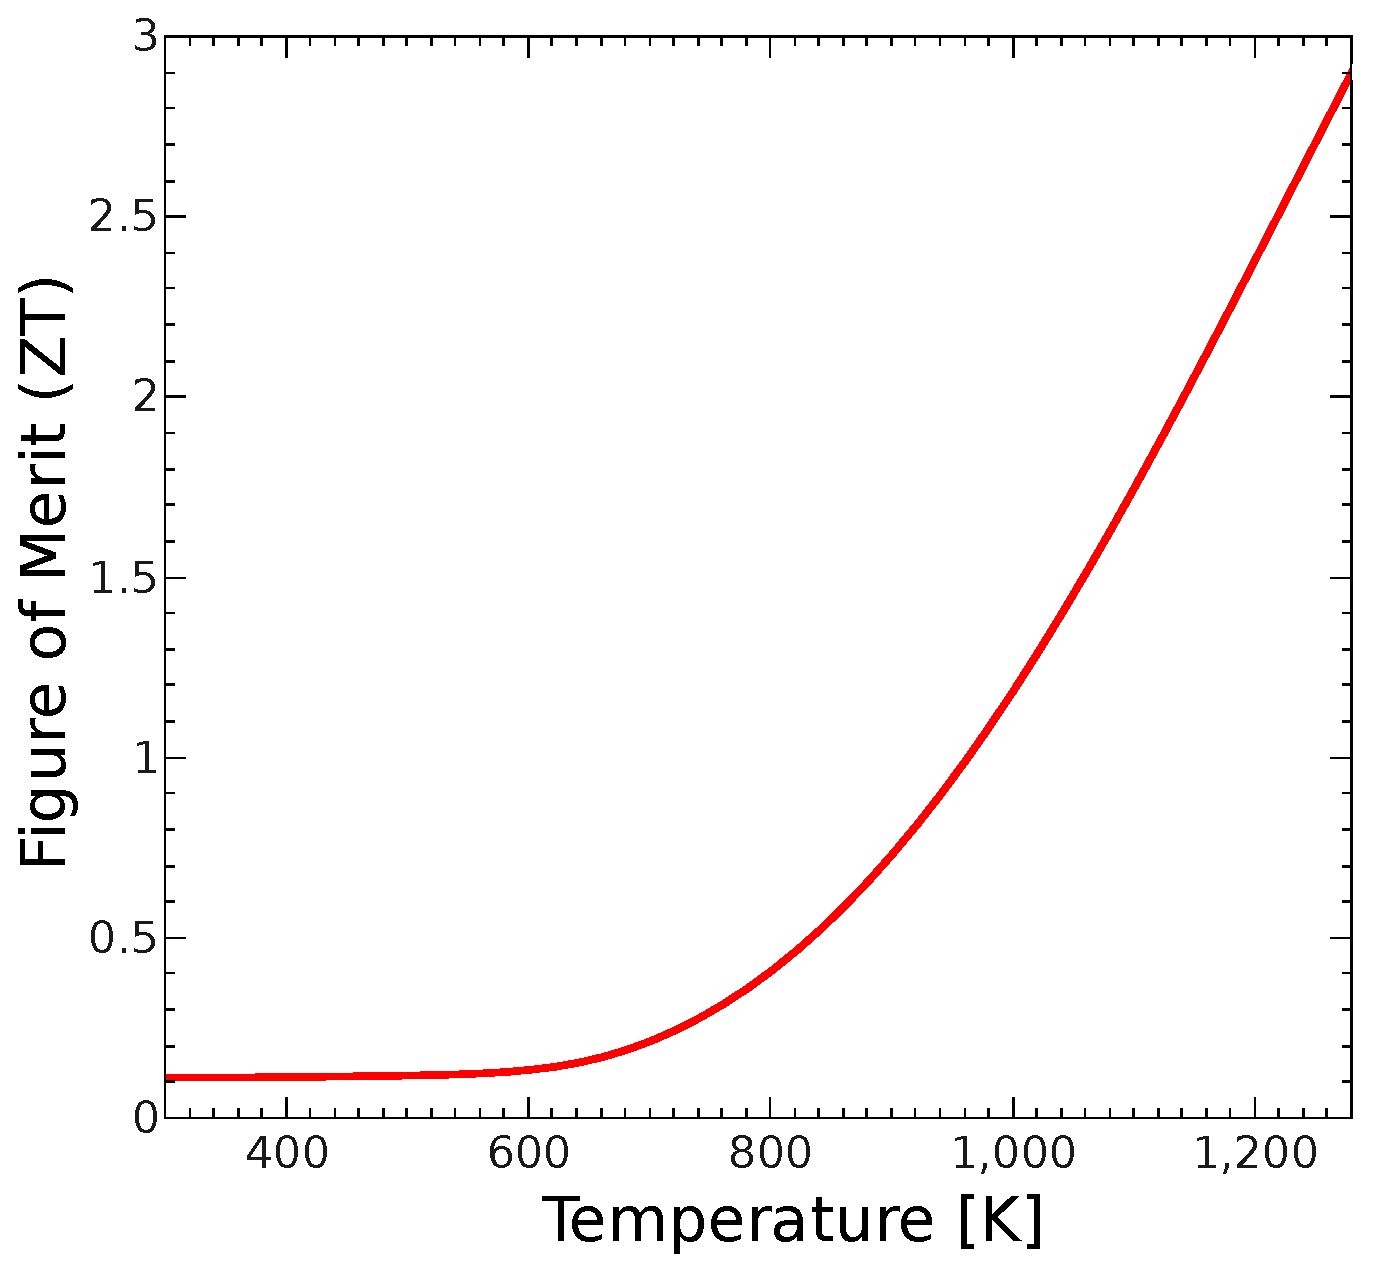
\includegraphics[width=0.8\textwidth]{ZT-10nm.eps}
	\caption{Zero-dimensional nanocomposite structure. Nanoscale spheres are densely packed with a homogeneous host material filling the voids. A temperature gradient is shown, to illustrate use as a thermoelectric.}
	\label{fig:zt-10nm}
\end{figure}

\section{Conclusion and Potential Development}
% Summarise results
% What else could be done?

% Link to your online repository
\url{https://github.com/kahlos/thermoelectrics}

% The {number} is related to the number of digits required for the references
\begin{thebibliography}{11}

\bibitem{modern-thermoelectrics}
D. M. Rowe,
\emph{Modern Thermoelectrics},
September 1983,
Holt-Technology,
ISBN:978-0835945936
\textbf{Page 12}

\bibitem{engine-efficiency}
M. L. Baglione,
\emph{Development of System Analysis Methodologies and Tools for Modeling and Optimizing Vehicle System Efficiency},
2007,
University of Michigan,
DOI:2027.42/57640
\textbf{Pages 52-54}

\bibitem{nanocomposite-zt}
R. Venkatasubramanian \emph{et al.},
\emph{Thin-film thermoelectric devices with high room-temperature figures of merit},
October 2001,
Nature, vol. 413, pp. 597-602,
DOI:10.1038/35098012

\bibitem{liu-review}
W. Liu \emph{et al.},
\emph{Recent advances in thermoelectric nanocomposites},
January 2012,
Nano Energy, vol. 1, iss. 1, pp. 42-56,
DOI:10.1016/j.nanoen.2011.10.001

\bibitem{solar-thermal}
D. Kraemer \emph{et al.},
\emph{High-performance flat-panel solar thermoelectric
generators with high thermal concentration},
May 2011,
Nature Materials 10, pp. 532-538,
DOI:10.1038/NMAT3013

\bibitem{exhust-recovery}
X. Liu \emph{et al.},
\emph{A case study on compatibility of automotive exhaust thermoelectric generation system, catalytic converter and muffler},
March 2014,
Case Studies in Thermal Engineering, vol. 2, pp. 62-66,
DOI:10.1016/j.csite.2014.01.002

\bibitem{thermo-cooling}
L. E. Bell,
\emph{Cooling, Heating, Generating Power, and Recovering Waste Heat with Thermoelectric Systems},
September 2008,
Science 12, vol. 321, no. 5895, pp. 1457-1461,
DOI:10.1126/science.1158899

\bibitem{minnich-review}
A. J. Minnich \emph{et al.},
\emph{Bulk nanostructured thermoelectric materials: current research and future prospects},
Feburary 2009,
Energy Environ. Sci. 2, pp. 466-479,
DOI:10.1039/B822664B

\bibitem{crc-handbook}
G. A. Slack, ed. D. M. Rowe,
\emph{CRC Handbook of Thermoelectrics},
1995,
CRC Press,
ISBN:978-0849301469
\textbf{Pages 407-440}

\bibitem{nanowires}
L. D. Hicks, M. S. Dresselhaus,
\emph{Thermoelectric figure of merit of a one-dimensional conductor},
June 1993,
Phys. Rev. B 47, 16631
DOI:10.1103/PhysRevB.47.16631

\bibitem{ema}
C. Nan \emph{et al.},
\emph{Effective thermal conductivity of particulate composites with interfacial thermal resistance},
February 1997,
Journal of Applied Physics 81, pp. 6692-6699,
DOI:10.1063/1.365209

\bibitem{phm}
L. Braginsky \emph{et al.},
\emph{High-temperature phonon thermal conductivity of nanostructures},
October 2002,
Physical Review B 66, 134203,
DOI:10.1103/PhysRevB.66.134203

\bibitem{kittel}
C. Kittel,
\emph{Introduction to Solid State Physics}, 8th Ed.,
November 2004,
John Wiley \& Sons,
ISBN:978-0471415268

\end{thebibliography}

\pagebreak

\appendix

\begin{center}
{\Huge\textbf{Appendix}}
\end{center}

\section{Further Questions and Thoughts}



\section{List of Assumptions}

\section{Further Reading}

\section{Tools and Software}

\section{Physical Data}

\section{Program Code}

\end{document}


